\documentclass{article}

\usepackage{amsmath}
\usepackage{ amssymb }
\usepackage{algorithm}
\usepackage{algpseudocode}
\usepackage{graphicx}
\usepackage{syntax}
\usepackage{tikz}
\usetikzlibrary{bayesnet}
\usetikzlibrary{arrows,automata, positioning, patterns,backgrounds}
\usetikzlibrary{arrows,shapes.gates.logic.US,shapes.gates.logic.IEC,calc}

\newcommand{\funtype}[2]{#1 \rightarrow #2}
\newcommand{\weightedrule}[3]{[#1 \mapsto #2 \, | \, #3]}
\newcommand{\typedexp}[2]{#1 : #2} 
\newcommand{\type}[1]{type(#1)}

\renewcommand{\grammarlabel}[2]{#1 #2}
\renewcommand{\given}{\, | \,}

\DeclareMathOperator*{\argmin}{argmin}
\DeclareMathOperator*{\argmax}{argmax}

\author{Eyal Dechter}
\begin{document}
\maketitle
\date

\section{Combinatory expressions as binary trees}
We use a polymorphic combinatory logic. Every combinatory logic
expression $e$ of type $\tau$ is defined to be either a primitive
combinator $c$ of type $\tau$ or the application of a left expression
$e_l$ of type $\funtype{\sigma}{\tau}$ to a right expression $e_r$ of
type $\sigma$ can be represented as a binary tree $t_e$, which
we call a \textbf{combinatory tree}. 

We define a stochastic process $\mathcal{D}$ that generates such
trees. A \textbf{terminal rule} $r = \weightedrule{\tau}{c}{w}$ specifies that a
nonterminal node of type $\tau$ can produce a primitive combinator $c$
with associated integer weight parameter $w$. $\mathcal{D}$ is a a set
of

\section{A stochastic grammar for polymorphic combinatory expressions}

A grammar for polymorphically typed combinatory expressions cannot be
context-free. To generate a function of type $t$, for example, I might
decide to apply a function of type $\funtype{s}{t}$ to an argument of
  type $s$. The types of the function and argument need to
  match. 

It is natural to describe a stochastic grammar in terms of the process
which generates elements from that grammar. To generate an expression
of type $t$, we begin with a nonterminal node of $t$:

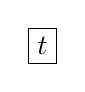
\begin{tikzpicture}
\node[draw]{$t$};
\end{tikzpicture}

We have two choices: 
\begin{enumerate}
\item (terminal production) With probability $p_{t \rightarrow c}$ we
  expand this node to terminal $c$ where $\type{c}$ unifies with $t$,
  and we update the type of the nonterminal to be the most general
  unifier (mgu) of $\type{c}$ and $t$:

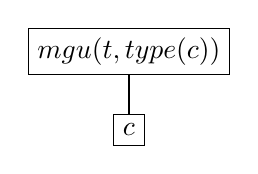
\begin{tikzpicture}
\node[draw](top){$mgu(t, \type{c})$};
\node[draw, below=.5cm of top](c){$c$};

\draw (top)--(c);
\end{tikzpicture}

We propogate this type up the expression tree. If we find a
nonterminal node that can be expanded, we procede with that
expansion. Otherwise, we are done.

\item (nonterminal production) With probability $p_{t \rightarrow
  \epsilon}$ we expand this node into an application:

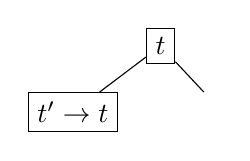
\begin{tikzpicture}
\node[draw](top){$t$};
\node[draw, below left=.5cm of top](left){$\funtype{t'}{t}$};
\node[below right=.5cm of top](right){};

\draw
(top) -- (left)
(top) -- (right);
\end{tikzpicture}
\end{enumerate}


Types:
\begin{grammar}
<$t$> ::= $\tau$, $\sigma$  (type variables)
  \alt $a$, $b$ (concrete types e.g. real, bool, int, etc.)
  \alt $\funtype{t'}{t}$ (function type)
\end{grammar}

Expressions: 
\begin{grammar}
<$\typedexp{e}{t}$> ::= $\typedexp{c}{t'}$ s.t. $t' = mgu(t,
\type{c})$ (substitute a terminal tree that unifies with the requesting type)
  \alt ($\typedexp{e}{\funtype{t'}{t}} \;\;\; \typedexp{e}{t'}$)
\end{grammar}

Let $G(e ; t)$ be the probability of type $t$ yielding expression
$e$. We define $G(\cdot \; ; \cdot)$ according to the following recursion:
\begin{align}
G( (e_1 \;\; e_2 ); t) &\propto \sum_{t' \trianglerighteq t} \phi_{t'} G(e_1 \; ; \; \funtype{s}{t})
   G(e_2 \; ; \;  \text{sourceType}(\type{e_1})\\
G( c \; ; \; t) &\propto \sum_{t' \trianglerighteq t} \phi_{\funtype{t'}{c}}
\end{align}



\section{A nonparametic prior over combinatory expressions}
We would like to describe a distribution over combinatory expressions
such that potential number of ``primitive combinators'' is
unbounded. This will allow us to naturally capture the possibility
that our library of combinator subroutines includes any number of
subroutines (themselves constructed of the primitive combinators). To
do this, we will use a modified version of the Pitman-Yor adaptor
grammar framework~\cite{DBLP:conf/nips/JohnsonGG06}. Our modification
is simply that instead of the base context-free grammar we use the
grammar described in the previous section. 

\section{E-C as MAP inference in a probabilistic graphical model.}
The motivation of the E-C algorithm is that a learning agent should
learn a library of useful program fragments that represents knowledge
about the kind the programs that are likely to solve problems in a
given domain. One way to frame this is as a probabilistic generative
model of the tasks that an agent encounters
(Figure~\ref{fig:generativeModel}).

\begin{figure}
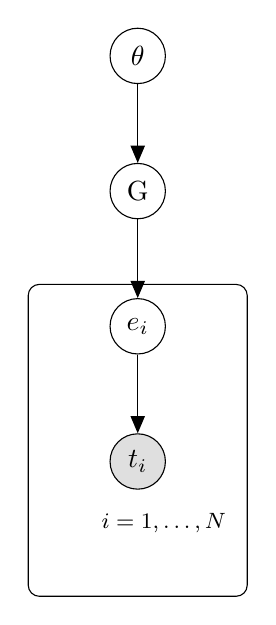
\begin{tikzpicture}[->, circle]

\node[latent] (theta) {$\theta$} ;
\node[latent, below=of theta] (G) {G} ;
\node[latent, below=of G]     (e) {$e_i$} ;
\node[obs, below=of e]     (t) {$t_i$} ;

\edge {theta} {G};
\edge {G} {e};
\edge {e} {t};

\plate {plate} {
  (e)(t)}{$i=1, \dots, N$};

\end{tikzpicture}
\caption{Generative model of program induction
  tasks. \label{fig:generativeModel}}
\end{figure}

Here each task $t_i$ is interpreted as a noisy version of the
underlying program $e_i$, and there is an associated likelihood
function $p_{t\given e}(t \given e) \propto f(t(e)) $ where $f$ is a monotonically
decreasing function. Given a task-specific loss function $t(\cdot)$, a
natural likelihood is $p_{t \given e}(t \given e) \propto \exp^{-t(e)}$. A set of
programs $\{e_i\}$ is drawn from a grammar $G$, which functions as the
subroutine library. Our prior expectations about $G$ are encoded in
$\theta$ via the distribution $p_{G \given \theta}$. 

The goal of the learner is the find the library $G$ and programs
$\{e_i\}$ that maximize $P(\{e_i\}, G \given  \{t_i\}, \theta)$. That is, 

\begin{align}
G^*, \{e^*_i\} &= \argmax_{G, \{e_i\} }
   P(\{e_i\}, G \given  \{t_i\}, \theta)\\
&= \argmax_{G, \{e_i\} }  P(\{t_i\} \given \{e_i\}) \;
  P(\{e_i\} \given G) \; P(G \given \theta)\\
&= \argmax_{G, \{e_i\} }
  \sum_i \left( 
  \log{p_{t\given e}\;(t_i \given e_i)}+ 
  \log{p_{e \given G}(e_i \given G)}
  \right ) +
  \log{p_{G \given \theta}\; (G \given \theta)}
\label{eq:objective}
\end{align}

The main difficulty in this optimization is that finding any candidate
program $e_i$ that provides a significant value for the first term is
difficult. If we knew $G$, we could sample programs from it as a way to
guide the search over the $e_i$. This suggests the following iterative
heuristic search algorithm. At iteration $j$, let $G^{(j)}$ be the
current best value of $G$. 

\begin{algorithm}
\caption{Hierarchical program induction (E-C)}\label{alg:basic-progind}
\begin{algorithmic}[1]
\State  \textbf{Exploration step: } Let $F$ be a set of $T$ samples
  i.i.d from $p_{e|G}(\cdot | G^{(j)})$.
\State \textbf{Compression step: } 
\begin{align*}
G^{(j+1)}, \{e^{(j+1)}_i\} &= 
\argmax_{G, \{e_i | e_i \in F \}}
\sum_i \left( 
\log{p_{t|e}(t_i|e_i)}+ 
\log{p_{e|G}(e_i|G)} \right )\\
&+
\log{p_{G|\theta}(G|\theta)}
\end{align*}
\end{algorithmic}
\end{algorithm}

\begin{enumerate}
\item \textbf{Exploration step: } Let $F$ be a set of $T$ samples
  i.i.d from $p_{e|G}(\cdot | G^{(j)})$.
\item \textbf{Compression step: } 
$$G^{(j+1)}, \{e^{(j+1)}_i\} = 
\argmax_{G, \{e_i | e_i \in F \}}
\sum_i \left( 
\log{p_{t|e}(t_i|e_i)}+ 
\log{p_{e|G}(e_i|G)}
\right ) +
\log{p_{G|\theta}(G|\theta)}
$$
\end{enumerate}

\subsection{An online algorithm}

Here we present an online version of the algorithm that only chooses
an expression for each task once. We can view the problem as MAP
estimation of the unobserved variables in the following graphical
model:

\begin{figure}[h]
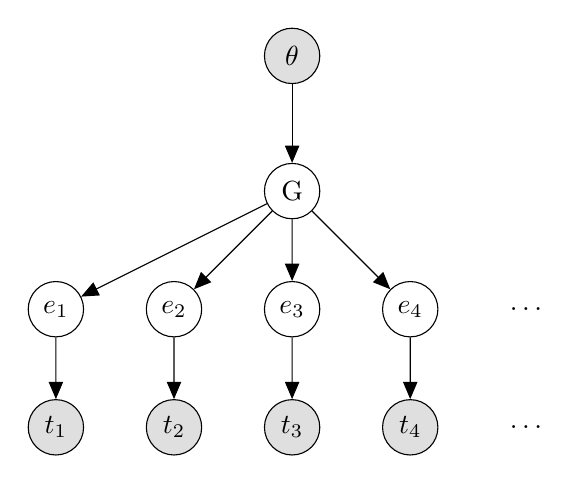
\begin{tikzpicture}[->, circle]

\node[obs] (theta) {$\theta$} ;
\node[latent, below=of theta] (G) {G} 
   child {node [latent] (e1) {$e_1$} 
      child {node [obs] (t1) {$t_1$}}}
   child {node [latent] (e2) {$e_2$} 
      child {node [obs] (t2) {$t_2$}}}
   child {node [latent] (e3) {$e_3$} 
      child {node [obs] (t3) {$t_3$}}}
   child {node [latent] (e4) {$e_4$} 
      child {node [obs] (t5) {$t_4$}}}
   child {node  (edots) {$\dots$} edge from parent[draw=none] 
      child {node  (tdots) {$\dots$} edge from parent[draw=none]}};


\edge {theta} {G};

\end{tikzpicture}
\end{figure}


We want to choose $e_i$ and $G$ to maximize our objective function. We
will perform the following iterative procedure. Given a current
setting of $G$, set $e_i$ to optimize the weights on the edges to
$t_i$ and $G$. Update $G$ to optimize the weight on the edge to
$\theta$ and all the edges to previous set expressions $e_j, j\leq
i$.

\begin{algorithm}
\caption{Online hierarchical program induction (version 1)}\label{alg:online-progind-v1}
\begin{algorithmic}
\State Initialize $G_0$.
\For{$i\gets 1, \dots$}
\State $e_i^* = \argmax_{e} \log p(t_i|e_i) + \log p(e_i|G_{i-1}) $
\State $G_i = \argmax_{G} \log p(G|\theta) + \sum_{j \leq i} \log p(e_j|G) $
\EndFor
\end{algorithmic}
\end{algorithm}


\begin{algorithm}
\caption{Online hierarchical program induction (version 2)}\label{alg:online-progind-v2}
\begin{algorithmic}
\State Initialize $G_0$.
\For{$i\gets 1, \dots$}
\State $F_i \sim \text{ i.i.d } p(\cdot | G)$
\State $e_i^* = \argmax_{e\in F_i} \log p(t_i|e_i) + \log p(e_i|G_{i-1}) $
\State $G_i = \argmax_{G} \log p(G|\theta) + \sum_{j \leq i} \log p(e_j|G) $
\EndFor
\end{algorithmic}
\end{algorithm}

\section{Combining planning with hierarchical program induction}
There is something clearly missing from this learning paradigm?
Actions, framed as programs acting on the environment, are not
proposed in a way that is contingent on the environment. But of course
the actions that we make are contingent on past behavior and sensory
input. A fundamental question, then, is how we can incorporate sensory
feedback and past behvarior into this learning paradigm. 

One answer to this is to combine planning with hierarchical program
induction. In this view, a solution to a problem is not a single
program. It is a series of programs, each of which attempts to get the
planner closer to the goal. The goal of the learner is to a learn a
distribution over programs that takes as input a sequence of past
actions and their effects and produces a new sequence of actions.

Let's consider a concrete example of such a domain: consider the
classic AI problem of stacking blocks to build a tower of a given
height. Let's make this problem somewhat more challenging by having
the agent build this tower on a vibrating platform. We define the
domain of primitive actions to be placing a block in either horizontal
or vertical orientation anywhere in a two dimensional vertical
plane. At any point during an attempted execution, the state of the
system is the sequence of previous primitive actions, and, perhaps,
auxiliary sensory information: in this case, an agent may make use of
the current configuration of blocks (i.e. what the tower looks like)
or some summary statistic thereof. We further assume that there is
some heuristic function (e.g. height) which guides the choice of the
next state.

Let $S$ be a state space and let $h:S \rightarrow \mathbb{R}$ be a
reward function. The planner's goal is to maximize the expected change
in reward of any given action $e \in \mathcal{L}$. Of course, the
change in reward does not only depend on the current action; it also
depends on the current state. But to simplify matters we will ignore
that for now, and assume that the state dependence is subsumed in the
distribution $p(\Delta h | e)$. That is, the planner wants to find
grammar $G^*$ such that
\begin{align}
G^* &= \argmax_G \sum_e \Delta h \;p(\Delta h | e) \, p(e|G) \, p(G|\theta).
\end{align}

As a first attempt to solve this problem, we can simply splice
Algorithm~\ref{alg:online-progind-v2} with a greedy actor who always
picks the best available action at any moment. Here, however, there is
only one ``task,'' and we are maximizing over only the grammar. This
is described in Algorithm~\ref{alg:planning-progind-v1}.

\begin{algorithm}
\caption{Planning with online program induction (version
  1)}\label{alg:planning-progind-v1}
\begin{algorithmic}
\State Initialize $G_0$.
\For{$i\gets 1, \dots$}
\State $F_i \sim \text{ i.i.d } p_{e|G}(\cdot | G_i)$
\State $G_i = \argmax_{G} \log p(G|\theta) 
+ \log \sum_{e_j \in F_0 \cup \dots \cup F_i}
\prod_{e_j} \Delta h(e_j) \; p(e_j|G) $
\State $e_i^* = \argmax_{F_i}$
\EndFor
\end{algorithmic}
\end{algorithm}












%% We can break this joint maximization into an iteration of
%% coordinate-wise maximization steps. First we fix $G$ and maximize the
%% programs, then we fix the programs and maximize $G$, repeating until
%% we are no longer improving out objective. This gives us the following
%% iterative algorithm, roughly corresponding to the indicated steps of
%% the E-C algorithm:

%% \begin{enumerate}
%% \item \textbf{Compression step} $$G^{(j+1)} = 
%%   \argmax_{G} \sum_i \left( 
%%   \log{p_{e|G}(e^{(j)}_i|G)}
%%   \right ) +
%%   \log{p_{G|\theta}(G|\theta)}$$
%% \item \textbf{Exploration step} $$\{e^{(j+1)}_i\} = 
%%   \argmax_{\{e_i\}}
%%   \sum_i \left( 
%%   \log{p_{t|e}(t_i|e_i)}+ 
%%   \log{p_{e|G}(e_i|G^{(j)})}
%%   \right ) $$
%% \end{enumerate}









\bibliographystyle{plain} \bibliography{grammar}


\end{document}
